\begin{figure}
\centering
\begin{tikzpicture}
  \node (circ) {
    \begin{tikzpicture}
      \node[inner sep=0pt] (circuit) {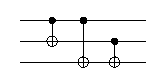
\includegraphics[scale=2]{Figures/circuits/bothEndsSimple}};  
      \node[above left=4.5mm and -7mm of circuit.west, opacity=0.9] {\footnotesize \(A\)};
      \node[left=-7mm of circuit.west, opacity=0.9] {\footnotesize \(B\)};
      \node[below left=4.5mm and -7mm of circuit.west, opacity=0.9] {\footnotesize \(C\)};
      \node[above right=0.8mm and 12.8mm of circuit.west, opacity=0.9] {\footnotesize \(\gamma\)};
      \node[below right=0.8mm and 23.6mm of circuit.west, opacity=0.9] {\footnotesize \(\beta\)};
      \node[below right=0.8mm and 34.4mm of circuit.west, opacity=0.9] {\footnotesize \(\alpha\)};
      \node[right=-3mm of circuit.north west, font=\itshape] (text) {a)};
    \end{tikzpicture}
  };
  \node[below left=5mm and -23mm of circ] (controlHyp) {
    \begin{tikzpicture}
      \coordinate (O) at (0,0);
      \coordinate (A) at (90:10mm);
      \coordinate (B) at (210:10mm);
      \coordinate (C) at (330:10mm);
      \draw (O) -- (A);
      \draw (O) -- (B);
      \draw (O) -- (C);
      \draw (B) -- (C);
      \node[circle, right=-2.5mm of A, fill=white, inner sep=0pt, minimum size=5mm] {\(A\)};
      \node[circle, right=-2.5mm of B, fill=white, inner sep=0pt, minimum size=5mm] {\(B\)};
      \node[circle, right=-2.5mm of C, fill=white, inner sep=0pt, minimum size=5mm] {\(C\)};
      \coordinate (leftPoint) at (270:10mm);
      \coordinate (rightPoint) at (30:10mm);
      \pic (cut) {cut=leftPoint/rightPoint};
      \node[above left=0mm and 13mm of A, font=\itshape] (text) {b)};
    \end{tikzpicture}
  };
  \node[right=8mm of controlHyp] (targetHyp) {
    \begin{tikzpicture}
      \coordinate (O) at (0,0);
      \coordinate (A) at (90:10mm);
      \coordinate (B) at (210:10mm);
      \coordinate (C) at (330:10mm);
      \draw[ultra thick] (O) -- (A);
      \draw[ultra thick] (O) -- (B);
      \draw[ultra thick] (O) -- (C);
      \draw[ultra thick] (A) -- (B);
      \node[circle, right=-2.5mm of A, fill=white, inner sep=0pt, minimum size=5mm] {\(A\)};
      \node[circle, right=-2.5mm of B, fill=white, inner sep=0pt, minimum size=5mm] {\(B\)};
      \node[circle, right=-2.5mm of C, fill=white, inner sep=0pt, minimum size=5mm] {\(C\)};
      \coordinate (leftPoint) at (270:10mm);
      \coordinate (rightPoint) at (30:10mm);
      \pic (cut) {cut=leftPoint/rightPoint};
      \node[above left=0mm and 13mm of A, font=\itshape] (text) {c)};
    \end{tikzpicture}
  };
  \node[below right=-20mm and 15mm of circ] (hypergraph) {
    \begin{tikzpicture}
      \coordinate (O) at (0,0);
      \coordinate (auxA) at (90:9mm);
      \coordinate (auxC) at (330:9mm);
      \coordinate (A) at (90:18mm);
      \coordinate (B) at (210:18mm);
      \coordinate (C) at (330:18mm);
      \coordinate (a) at (270:9mm);
      \coordinate (b) at (30:9mm);
      \coordinate (c) at (150:9mm);
      \draw (auxA) -- (A);
      \draw (auxA) -- (b);
      \draw (auxA) -- (c);
      \draw[ultra thick] (auxC) -- (C);
      \draw[ultra thick] (auxC) -- (b);
      \draw[ultra thick] (auxC) -- (a);
      \draw (B) -- (a);
      \draw[ultra thick] (B) -- (c);
      \node[circle, right=-2.5mm of A, fill=white, inner sep=0pt, minimum size=5mm] {\(A\)};
      \node[circle, right=-2.5mm of B, fill=white, inner sep=0pt, minimum size=5mm] {\(B\)};
      \node[circle, right=-2.5mm of C, fill=white, inner sep=0pt, minimum size=5mm] {\(C\)};
      \node[circle, right=-2.5mm of a, fill=white, inner sep=0pt, minimum size=5mm] {\(\alpha\)};
      \node[circle, right=-2.5mm of b, fill=white, inner sep=0pt, minimum size=5mm] {\(\beta\)};
      \node[circle, right=-2.5mm of c, fill=white, inner sep=0pt, minimum size=5mm] {\(\gamma\)};
      \coordinate (leftPoint) at (285:18mm);
      \coordinate (rightPoint) at (15:18mm);
      \pic (cut) {cut=leftPoint/rightPoint};
      \node[above left=0mm and 13mm of A, font=\itshape] (text) {d)};
    \end{tikzpicture}
  };
\end{tikzpicture}
%\vspace*{5mm}
\caption{A circuit \textit{a)} and its hypergraph \textit{b)} as built by Algorithm~\ref{code:buildHypVanilla}. Hypergraph \textit{c)} is the result of running the same algorithm but grouping CNOTs in the same hyperedge if and only if they share the same target (instead of control). Hypergraph \textit{d)} is the one built by Algorithm~\ref{code:buildHypBothEnds}.}
\label{fig:BothEndsChallenge}
\end{figure}